
\section{Anforderungsspezifikation}
\label{Anforderungsspezifikation}

\subsection{Use Cases}
\label{Anforderungsspezifikation:Use Cases}

Im Folgenden sind die funktionalen Anforderungen an das System mit all seinen Komponenten, welche im Kapitel \ref{Architektur} aufgeführt sind, als Use Cases im Brief-Format beschrieben.
Zur Übersicht ist das Use Case Diagramm in Abbildung \ref{fig:UseCase_OeV-Gueteklassen_2018} zu betrachten.

\begin{figure}[ht]
\centering
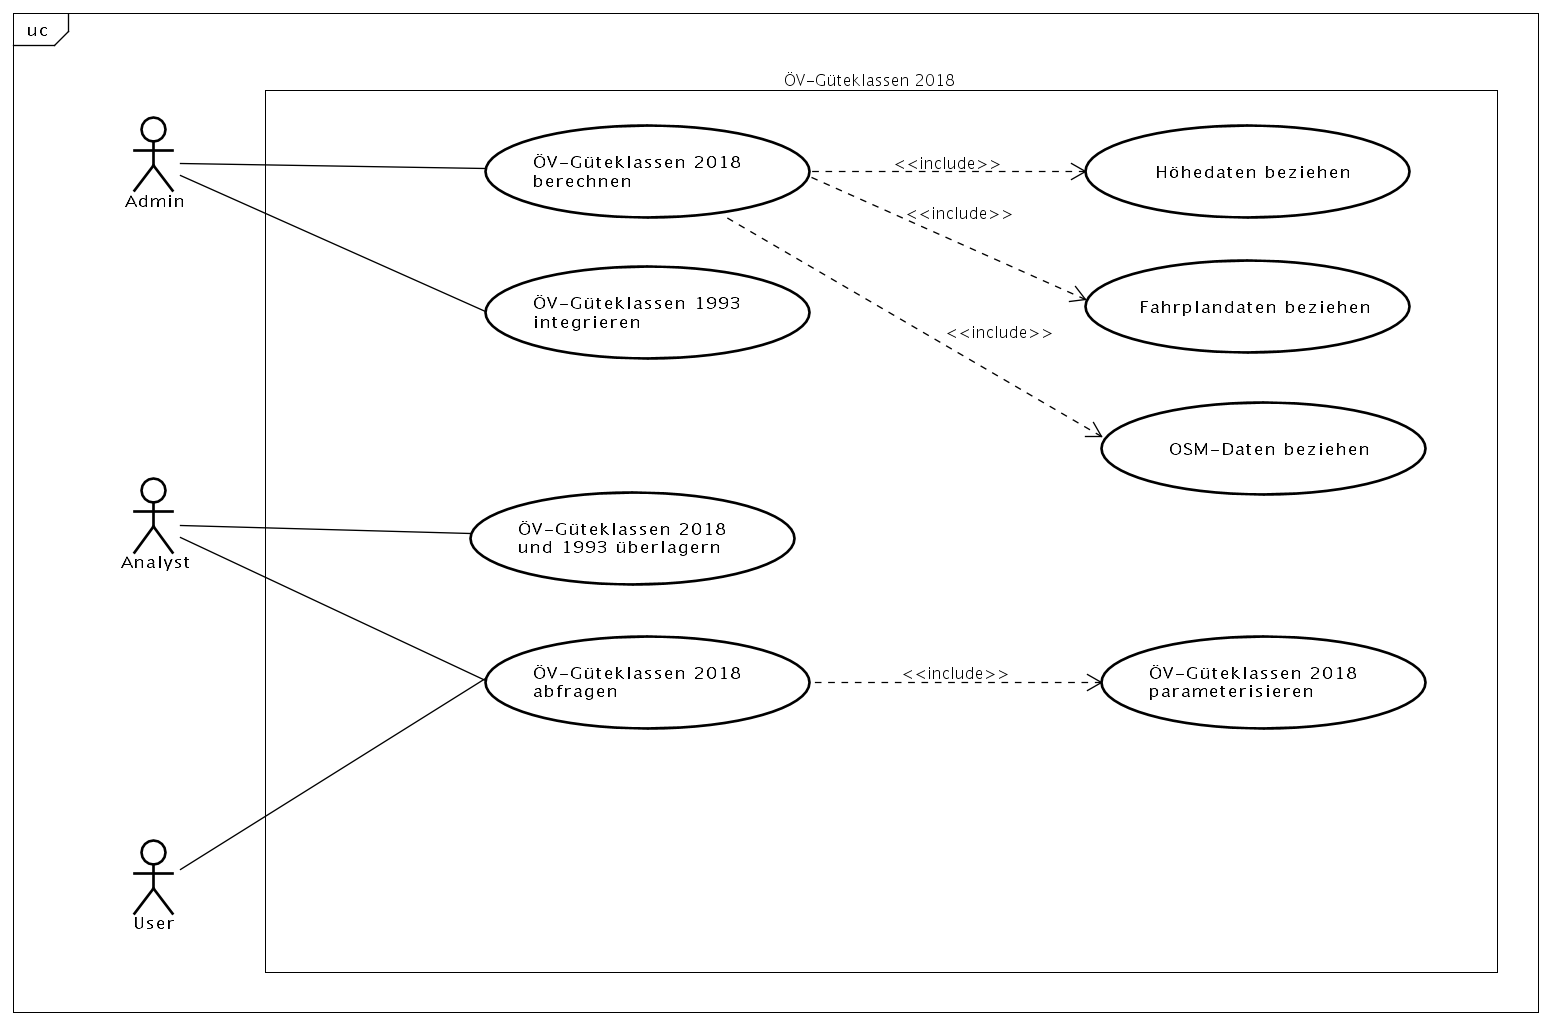
\includegraphics[width=1.0\linewidth]{projectdoc/img/UseCase_OeV-Gueteklassen_2018}
\caption[Use Case Diagramm]{Use Case Diagramm}
\label{fig:UseCase_OeV-Gueteklassen_2018}
\end{figure}

\subsubsection{Aktoren}
\label{Use Cases:Aktoren}

Um die Anforderungen akkurat evaluieren zu können, ist es essentiell, die Aktoren des Systems zu identifizieren.
In der Tabelle \ref{table:Aktoren} sind die Aktoren mit ihren Interessen aufgelistet.

\begin{longtable}{l p{14cm}}
        \toprule
        \textbf{Aktor}
                                & \textbf{Beschreibung und Interesse} \\
        \midrule
        \textbf{Admin}
                                & Ein \emph{Admin} ist für die Bereitstellung von akkuraten \acs{ÖV}-Güteklassen-Daten verantwortlich, welche er den Aktoren \emph{Analyst} und \emph{User} für die weitere Auswertung zur Verfügung stellt.
                                So möchte er die erforderlichen Daten sammeln und verarbeiten. \\
        \textbf{Analyst}
                                & Unter dem Aktor \emph{Analyst} sind Raum-/Verkehrsplaner, Transportgesellschaften und weitere Personen zusammengefasst, welche die \acs{ÖV}-Güteklassen-Daten für analytische Zwecke und als Planungsinstrument verwenden möchten. \\
        \textbf{User}
                                & Ein \emph{User} ist grundsätzlich am aktuellen Stand der \acs{ÖV}-Güteklassen in einer bestimmten Region interessiert, welche er als Basis für weitere Entscheidungen bezieht. \\
        \bottomrule
    \caption{Aktoren}
    \label{table:Aktoren}
\end{longtable}

\subsubsection{UC01: ÖV-Güteklassen 2018 berechnen}
\label{Use Cases:UC01}

Aktoren: \emph{Admin}

Include: \nameref{Use Cases:UC02}, \nameref{Use Cases:UC03}, \nameref{Use Cases:UC04}

Der \emph{Admin} startet die Berechnung der \acs{ÖV}-Güteklassen 2018 basierend auf einer Konfiguration (Stichtage und Zeitspannen) periodisch.


\subsubsection{UC02: Höhendaten vorverarbeiten}
\label{Use Cases:UC02}

Aktoren: \emph{Admin}

Der \emph{Admin} füḧrt das manuelle Beziehen der Höhendaten durch und übergibt diese dem System ''\acs{ÖV}-Güteklassen 2018''.
Das System bereit die Daten so vor, dass sie in \nameref{Use Cases:UC01} für die ''\acs{ÖV}-Güteklassen 2018''-Berechnung einbezogen werden können
Da die diese Daten nicht einem stetigen Wandel unterstehen, steht es dem \emph{Admin} frei, diesen Schritt auszulassen und bereits im System vorhandene, verarbeitete Höhendaten zu verwenden.

\subsubsection{UC03: Fahrplandaten periodisch vorverarbeiten}
\label{Use Cases:UC03}

Aktoren: \emph{Admin}

Der \emph{Admin} nutzt das System ''\acs{ÖV}-Güteklassen 2018'' für das periodische Beziehen der Fahrplandaten über eine externe Schnittstelle.
Das System bereit die Daten so vor, dass sie in \nameref{Use Cases:UC01} für die ''\acs{ÖV}-Güteklassen 2018''-Berechnung einbezogen werden können.

\subsubsection{UC04: OSM-Daten periodisch vorverarbeiten}
\label{Use Cases:UC04}

Aktoren: \emph{Admin}

Der \emph{Admin} nutzt das System ''\acs{ÖV}-Güteklassen 2018'' für das periodische Beziehen der \acs{OSM}-Daten über eine externe Schnittstelle.
Das System bereit die Daten so vor, dass sie in \nameref{Use Cases:UC01} für die ''\acs{ÖV}-Güteklassen 2018''-Berechnung einbezogen werden können.


\subsubsection{UC05: ÖV-Güteklassen 1993 integrieren}
\label{Use Cases:UC05}

Aktoren: \emph{Admin}

Der \emph{Admin} nutzt das System ''\acs{ÖV}-Güteklassen 2018'' für die Integration der bereits berechneten ÖV-Güteklassen 1993~\cite{berechnung_are}.


\subsubsection{UC06: ÖV-Güteklassen 2018 und 1993 vergleichen}
\label{Use Cases:UC06}

Aktoren: \emph{Analyst}

Der \emph{Analyst} nutzt das System ''\acs{ÖV}-Güteklassen 2018'' für den Vergleich der \acs{ÖV}-Güteklassen 1993 und 2018.
Das System präsentiert eine grafische Überlagerung der beiden \acs{ÖV}-Güteklassen.

\subsubsection{UC07: ÖV-Güteklassen 2018 abfragen}
\label{Use Cases:UC07}

Aktoren: \emph{Analyst, User}

Include: \nameref{Use Cases:UC08}

Die Aktoren \emph{Analyst} und \emph{User} nutzt das System ''\acs{ÖV}-Güteklassen 2018'', um die berechneten \acs{ÖV}-Güteklassen 2018 anzuzeigen.


\subsubsection{UC08: ÖV-Güteklassen 2018 parametrisieren}
\label{Use Cases:UC08}

Aktoren: \emph{Analyst, User}

Die Aktoren \emph{Analyst} und \emph{User} übergibt dem System ''\acs{ÖV}-Güteklassen 2018'' eine Konfiguration der anzuzeigenden \acs{ÖV}-Güteklassen 2018.
Das System ''\acs{ÖV}-Güteklassen 2018'' liefert auf Basis dieser die zugehörigen, vorgerechneten Daten.

\subsection{Nicht-funktionale Anforderungen}
\label{Anforderungsspezifikation:Nicht-funktionale Anforderungen}

Im Folgenden sind die nicht-funktionale Anforderungen an das System ''\acs{ÖV}-Güteklassen 2018'' aufgelistet.
Bei der Erarbeitung wird darauf geachtet, dass die Kriterien \emph{Specific} und \emph{Measurable} aus den \emph{SMART}-Kriterien~\cite{SMART} eingehalten werden.
Als Spezifikation-Template wird das bewährte Quality Attribute Scenario (QAS) des Software Engineering Institute (SEI)~\cite{BassSoftwareArchitecture2012} eingesetzt.
In der Kategorie \emph{Stimulus Source} werden die Aktoren aus der Tabelle \ref{table:Aktoren} wiederverwendet.
Die erwähnten Komponenten sind im Kapitel \ref{Architektur} genauer beschrieben.

\subsubsection{NFA01: Auslieferung der Komponenten als Docker-Image}
\label{NFA:NFA01}

\begin{longtable}{l p{10.6cm}}
        \toprule
        \textbf{Scenario}
                                & Auslieferung der Komponenten als Docker-Image\\
        \midrule
        \textbf{Business Goals}
                                & Deployment und Portierbarkeit gewährleisten \\
        \textbf{Relevant Quality Attributes}
                                & Maintainability, Manageability, Portability, Deployability\\
        \textbf{Stimulus Source}
                                & Admin\\
        \textbf{Stimulus}
                                & Die Generierung des Docker-Image wird gestartet\\
        \textbf{Environment}
                                & Normaler Betrieb (unabhängig vom laufenden Web-App und Backend)\\
        \textbf{Artifact}
                                & Das ganze System ''ÖV-Güteklassen 2018'' mit all seinen Komponenten\\
        \textbf{Response}
                                & Die Komponenten sind als Docker-Images verfügbar, welche auf Docker Hub hochgeladen werden könnten\\  
        \textbf{Response Measure}
                                & Einzelne Komponenten lassen sich als Docker-Image starten\\
                                  
        \bottomrule
    \caption{QAS NFA01}
    \label{table:nfa01}
\end{longtable}

\subsubsection{NFA02: Berechnung der ÖV-Güteklassen 2018}
\label{NFA:NFA02}

\begin{longtable}{l p{10.6cm}}
        \toprule
        \textbf{Scenario}
                                & Berechnung der ÖV-Güteklassen 2018\\
        \midrule
        \textbf{Business Goals}
                                & Aktualisierte ÖV-Güteklassen 2018 für weitere Auswertungen\\
        \textbf{Relevant Quality Attributes}
                                & Performance (response time), Usability, Manageability\\
        \textbf{Stimulus Source}
                                & Admin\\
        \textbf{Stimulus}
                                & Ausführung \nameref{Use Cases:UC01}\\
        \textbf{Environment}
                                & Normaler Betrieb (unabhängig vom laufenden Web-App und Backend)\\
        \textbf{Artifact}
                                & ÖV-Güteklassen 2018 Processor und seine abhängige Fremdsysteme\\
        \textbf{Response}
                                & Berechnete ÖV-Güteklassen 2018 als GeoJSON\\  
        \textbf{Response Measure}
                                & Die ÖV-Güteklassen 2018 lassen sich innerhalb von 2 Stunden nach Absetzen des Befehls über ein CLI berechnen\\                                
        \bottomrule
    \caption{QAS NFA02}
    \label{table:nfa02}
\end{longtable}

\subsubsection{NFA03: Periodische Aktualisierung der ÖV-Güteklassen 2018}
\label{NFA:NFA03}

\begin{longtable}{l p{10.6cm}}
        \toprule
        \textbf{Scenario}
                                & Periodische Aktualisierung der ÖV-Güteklassen 2018\\
        \midrule
        \textbf{Business Goals}
                                & Automatisch aktualisierte ÖV-Güteklassen 2018 für weitere Auswertungen\\
        \textbf{Relevant Quality Attributes}
                                & Administrability\\
        \textbf{Stimulus Source}
                                & Cron-Job\\
        \textbf{Stimulus}
                                & Periodische Ausführung \nameref{Use Cases:UC01} \\
        \textbf{Environment}
                                & Normaler Betrieb (unabhängig vom laufenden Web-App und Backend)\\
        \textbf{Artifact}
                                & ÖV-Güteklassen 2018 Processor und seine abhängige Fremdsysteme\\
        \textbf{Response}
                                & Berechnete ÖV-Güteklassen 2018 als GeoJSON\\  
        \textbf{Response Measure}
                                & Alle zwei Wochen liegt ein aktualisiertes GeoJSON bereit, welches von anderen Komponenten verwendet werden kann\\
        \bottomrule
    \caption{QAS NFA03}
    \label{table:nfa03}
\end{longtable}

\subsubsection{NFA04: Dauer des Unterbruchs bei Integration aktualisierter Daten}
\label{NFA:NFA04}

\begin{longtable}{l p{10.6cm}}
        \toprule
        \textbf{Scenario}
                                & Dauer des Unterbruchs bei Integration aktualisierter Daten\\
        \midrule
        \textbf{Business Goals}
                                & Kurzer Unterbruch während des Einspielens aktualisierter Daten\\
        \textbf{Relevant Quality Attributes}
                                & Availability \\
        \textbf{Stimulus Source}
                                & Admin\\
        \textbf{Stimulus}
                                & Nach Ausführung von \nameref{Use Cases:UC01} und \nameref{Use Cases:UC05} durch manuelle Interaktion des Admin\\
        \textbf{Environment}
                                & Web-App und Backend ist heruntergefahren\\
        \textbf{Artifact}
                                & Web-App und Backend\\
        \textbf{Response}
                                & Web-App ist wieder verfügbar und Backend ist mit aktualisierten ''ÖV-Güteklassen 2018''-Daten gestartet\\  
        \textbf{Response Measure}
                                & Web-App ist nicht länger als eine Stunde vom Zeitpunkt des Herunterfahrens nicht verfügbar\\                                
        \bottomrule
    \caption{QAS NFA04}
    \label{table:nfa04}
\end{longtable}

\subsubsection{NFA05: Antwortzeit ÖV-Güteklassen 2018 anzeigen}
\label{NFA:NFA05}

\begin{longtable}{l p{10.6cm}}
        \toprule
        \textbf{Scenario}
                                & Antwortzeit ÖV-Güteklassen 2018 anzeigen\\
        \midrule
        \textbf{Business Goals}
                                & \\
        \textbf{Relevant Quality Attributes}
                                & Performance (response time), Scalability\\
        \textbf{Stimulus Source}
                                & User, Analyst\\
        \textbf{Stimulus}
                                & Ausführung \nameref{Use Cases:UC06} oder \nameref{Use Cases:UC07}\\
        \textbf{Environment}
                                & Normaler Betrieb\\
        \textbf{Artifact}
                                & Web-App und Backend\\
        \textbf{Response}
                                & ÖV-Güteklassen 2018 werden für den gewünschten Bereich angezeigt\\  
        \textbf{Response Measure}
                                & ÖV-Güteklassen 2018 werden nach Verändern des Zooms innerhalb von 5 Sekunden angezeigt\\
        \bottomrule
    \caption{QAS NFA05}
    \label{table:nfa05}
\end{longtable}
